\documentclass[utf8x, 14pt]{article}

\usepackage{graphicx}

\usepackage{listings}
% https://tex.stackexchange.com/questions/108692/listing-with-mixed-english-and-russian-symbols-in-comments
\lstdefinestyle{CppCodeStyle}{
	basicstyle=\footnotesize\ttfamily,
	language={[ANSI]C++},
	keywordstyle=\bfseries,
	showstringspaces=false,
	morekeywords={include, printf},
	commentstyle={},
	texcl=true,     %<---- added
}

\usepackage{hyperref}

% https://tex.stackexchange.com/questions/816/cyrillic-in-latex
\usepackage[utf8]{inputenc}
\usepackage[russian]{babel}
% https://tex.stackexchange.com/questions/6260/how-to-draw-box-around-text-that-contains-a-verbatim-block
\usepackage{fancyvrb}
% https://www.sharelatex.com/learn/Page_size_and_margins
\usepackage[a4paper, total={6in, 9in}]{geometry}

\begin{document}
	
\begin{center} 
	
	\large Санкт-Петербургский политехнический университет \\Петра Великого\\
	Институт компьютерных наук и технологий\\
	Кафедра компьютерных систем и программных технологий\\[5.5cm] 
	
	\huge Отчёт по курсовому проекту \\[0.6cm] % название работы, затем отступ 0,6см
	\large по дисциплине: <<Параллельные вычисления>>\\[3.7cm]
	
	
\end{center} 

%\begin{flushright}
%Выполнил: студент гр.  13541/3\\
%В.Ю. Григорьев \\
%Руководитель:\\
%А.М. Сазанов
%\end{flushright}
\newbox{\lbox}
\savebox{\lbox}{\hbox{И.В. Стручков}}
\newlength{\maxl}
\setlength{\maxl}{\wd\lbox}
\hfill\parbox{10cm}{
	\hspace*{4cm}\hspace*{-4cm}Студент гр. 13541/3:\hfill\hbox to\maxl{В.Ю. Григорьев\hfill}\\
	\hspace*{4cm}\hspace*{-4cm}Руководитель:\hfill\hbox to\maxl{И.В. Стручков}\\
	\newline
	\hspace*{5cm}“\underline{\qquad}” \underline{\qquad\qquad} 2018 г.\\
	\\
}

\vfill 

\begin{center} 
	\large Санкт-Петербург\\2018
\end{center} 

\thispagestyle{empty}
\newpage

\tableofcontents

\newpage

\section{Постановка задачи}
В данной работе необходимо:
\begin{enumerate}
	\item разработать программу, реализующую алгоритм Беллмана-Форда на языка C++
	\item протестировать полученное решение
	\item провести анализ полученного алгоритма, выделить части, которые могут быть распараллелены, разработать структуру параллельной программы
	\item реализовать параллельную программу и проверить её на созданном ранее наборе тестов
	\item реализовать алгоритм Беллмана-Форда и его параллельный вариант с использованием средств языка на выбор
	\item провести эксперименты для оценки времени выполнения последовательной и параллельной программ, проанализировать полученные результаты
\end{enumerate}

\section{Введение}
Алгоритм Беллмана-Форда — алгоритм поиска кратчайшего пути во взвешенном графе. Алгоритм находит кратчайшие пути от одной вершины графа до всех остальных. 

\section{Ход работы}
\subsection{Разработка программы на языке C++}

На основании данного псевдокода

\begin{figure}[h!]
	\centering
	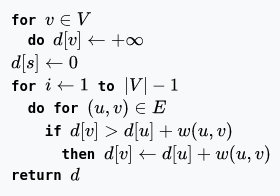
\includegraphics[scale=0.75]{Bellman-Ford.png}
	\caption{Псевдокод алгоритма Беллмана-Форда}
\end{figure}

и неформального описания алгоритма\cite{algo} была создана программа на языке C++, реализующая данный алгоритм.
\newpage
\begin{lstlisting}[language=C++, numbers=left, frame=single]
void solve() {
	vector<int> d (n, INF);
	d[v] = 0;

	for (int i=0; i<n-1; i++) {
		for (int j=0; j<m; j++)
			if (d[e[j].a] < INF) {
				if (d[e[j].b] > d[e[j].a] + e[j].cost) {
					d[e[j].b] = d[e[j].a] + e[j].cost;
				}
			}
	}
}
\end{lstlisting}

Полный код программы представлен в Приложении 1.

Здесь \textbf{вектор d} - вектор, где \textbf{d}[\textit{node-index}] содержит путь от стартовой вершины до вершины с номером \textit{node-index}.

\textbf{e} - вектор, содержащий описание всех граней (задаётся в файле и не меняется на протяжении работы программы). \textbf{a} - вершина, из которой выходит грань, \textbf{b} - вершина, в которую входит грань, \textbf{cost} - цена грани.

\textbf{n} - количество вершин, \textbf{m} - количество граней.

\subsubsection{Формат хранения графа}
В качестве способа хранения графа был выбран формат CSV.

В первой строке находятся 4 числа:
\begin{enumerate}
	\item кол-во вершин
	\item кол-во граней
	\item номер начальной вершины
	\item номер конечной вершины
\end{enumerate}

В следующих строках находится описание граней:
\begin{enumerate}
	\item номер вершины, откуда выходит грань
	\item номер вершины, куда идёт грань
	\item цена грани
\end{enumerate}

Пример:

\begin{tabular}{c}
	\begin{lstlisting}
				6,8,0,3
				0,1,10
				0,5,8
				1,3,2
				2,1,1
				3,2,-2
				4,1,-4
				4,3,-1
				5,4,1
	\end{lstlisting}
\end{tabular}

\newpage
Таким образом задаётся данный граф:

\begin{figure}[h!]
	\centering
	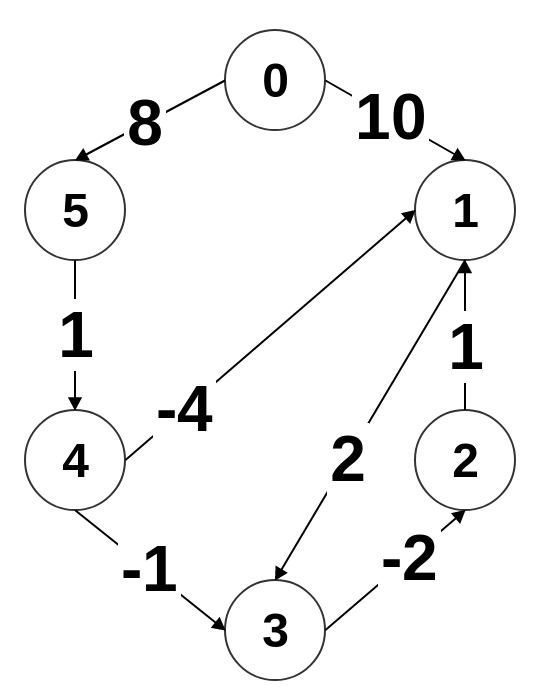
\includegraphics[scale=0.5]{graph.png}
	\caption{Граф}
\end{figure}

Пробуем <<решить>> данный граф с помощью написанной программы:

\begin{lstlisting}[frame=single]
Time passed: 4.192e-06
Path from 0 to 3: 
0 5 4 1 3 
\end{lstlisting}

Если попробовать найти путь вручную, ответ получится таким же, что позволяет заключить о правильной работе написанного алгоритма.

\subsection{Разработка скрипта для генерации графов}
Однако, на таких простых графах программа отрабатывает слишком быстро, чтобы можно было измерять и рассчитывать изменения времени её выполнения.

Чтобы довести время работы программы до значимых величин, необходимо подавать ей гораздо более сложные графы. В открытом доступе не было найдено решений под эту задачу, поэтому было принято решение написать скрипт, случайно генерирующий ориентированные графы.

\begin{lstlisting}[language=Python, frame=single, breaklines=true]
import argparse
import csv
import random


class Matrix:
	def __init__(self, mat, nodes_num, connections_num):
		self.mat = mat
		self.nodes_num = nodes_num
		self.connections_num = connections_num


def generate_graph_matrix(n, edge_chance):
	# Matrix n*n
	mat = [[0 for _ in range(n)] for _ in range(n)]
	
	connections = 0
	
	for i in range(n):
		for j in range(n):
			if i == j:
				continue
			connection_weight = None
			if random.random() <= edge_chance:
				connections += 1
				mat[i][j]= random.randint(1, 10)
	
	return Matrix(mat, n, connections)


def save_graph_from_matrix(matrix, file, start, end):
	with open(file, 'wt', newline='') as csv_file:
		writer = csv.writer(csv_file)
		writer.writerow([matrix.nodes_num, matrix.connections_num, start, end])
		
		mat = matrix.mat
		for i in range(matrix.nodes_num):
			for j in range(matrix.nodes_num):
				if mat[i][j] != 0:
					writer.writerow([i, j, mat[i][j]])


if __name__ == '__main__':
	parser = argparse.ArgumentParser(description="Generate graph.")
	parser.add_argument('nodes', type=int, help="Number of nodes in graph.")
	parser.add_argument('edge_chance', type=float, help="Chance to spawn edge for two nodes. This basically means that there will be approx. (n*n*edge_chance) edges in the graph.")
	parser.add_argument('output_file', help="Output file.")
	parser.add_argument('-s', '--start_node', type=int, help="Start node index.")
	parser.add_argument('-e', '--end_node', type=int, help="End node index.")
	parser.add_argument('-k', '--key', help="Seed for RNG.")
	
	args = parser.parse_args()
	
	if args.key:
		# Repeatable random
		random.seed(args.key)
		
	matrix = generate_graph_matrix(args.nodes, args.edge_chance)
	
	start_node = args.start_node or 1
	end_node = args.end_node or (args.nodes - 1)
	save_graph_from_matrix(matrix, args.output_file, start_node, end_node)
	
	print(f"Graph generated and saved in {args.output_file}")
\end{lstlisting}

Данный скрипт случайно заполняет матрицу смежности на основании переданных аргументов командной строки и сохраняет полученный граф в CSV формате.

\subsection{Распараллеливание алгоритма}

В написанном алгоритме явно выделяется часть, которая может быть легко распараллелена - вложенный цикл, проходящий по всем граням. Значение каждой итерации данного цикла не зависит от значения предыдущей, соответственно, их можно выполнять не последовательно, а в параллель.

\begin{lstlisting}[language=C++, numbers=left, frame=single]
void solve() {
  vector<int> d (n, INF);
  d[v] = 0;
	
  for (int i=0; i<n-1; i++) {
	#pragma omp parallel for
	for (int j=0; j<m; j++)
	  if (d[e[j].a] < INF) {
		if (d[e[j].b] > d[e[j].a] + e[j].cost) {
		  d[e[j].b] = d[e[j].a] + e[j].cost;
		}
	  }
	}
}
\end{lstlisting}

Это легко достигается с помощью директивы \textit{\#pragma omp parallel for} над интересующим нас циклом.

Может показаться, что при данном подходе возникает риск появления состояний гонки из-за того, что каждая итерация может записать в вектор d.

Однако, учитывая работу алгоритма, не имеет значения, если в итоге будет записана не самая маленькая величина. Количество итераций внешнего цикла (n-1) всё равно достаточно для того, чтобы в итоге все пути получились наименьшими.

Ситуации же, когда два потока одновременно попытаются записать значение в одну и ту же ячейку (получив torn write), не возникнет, так как запись в 32-битное значение (DWORD) на х86 атомарно\cite{intel}.

Таким образом, шанс получить отличающийся от последовательной программы ответ существует лишь в случае, когда в графе есть два кратчайших маршрута с одинаковой стоимостью, что не может считаться некорректной работой программы.

Тестируем параллельную программу на том же графе:

\begin{lstlisting}[frame=single]
Time passed: 0.000243342
Path from 0 to 3: 
0 5 4 1 3 
\end{lstlisting}

Результат получился идентичным, что позволяет судить о правильной работе программы.

\subsection{Реализация параллельности средствами языка}

Для второй части работы было принято решение реализовать алгоритм в функциональном стиле, чтобы обеспечить возможность распараллеливания простой заменой \textbf{map} на \textbf{pmap}(параллельный map).

В качестве языка для реализации был выбран \textbf{Clojure}, т.к. это язык с превалирующей функциональной парадигмой с простым синтаксисом (Lisp) и JVM в качестве backend-платформы.

\begin{lstlisting}[language=Lisp, frame=single]
(defn relax-nodes [edges-list nodes]

  (defn calc-cost [edge]

	(let [[start-cost _] (get nodes (:a edge))
          [end-cost old-parent] (get nodes (:b edge))]
	  (if (< (+ start-cost (:cost edge)) end-cost)
		[(+ start-cost (:cost edge)) (:a edge)]
		[end-cost old-parent])))
	
  (defn relax-each [node edges-for-node]

	(if (zero? (first node))
	  [0 0]
	  (apply min-key first (map calc-cost edges-for-node))))

  (into [] (map relax-each nodes edges-list)))

(defn bellman-ford [nodes-num start-node edges-list]

  (let [inf-src (repeat Double/POSITIVE_INFINITY)]
	(->>
	  (map vector
	  (flatten [(take start-node inf-src) 0 
	    (take (- nodes-num start-node) inf-src)])
	  (take nodes-num (repeat 0)))
	  (into [])
	  (iterate (partial relax-nodes edges-list))
	  (take (- nodes-num 1))
	  last
	  time)))
\end{lstlisting}

Полный код программы приведён в Приложении 2.

Как видно из кода программы, все функции, занимающиеся непосредственно вычислением - чистые, а все структуры в Clojure - персистентные.

Комбинация вышесказанного позволяет добиться параллельной работы программы с помощью простой замены \textbf{map} на \textbf{pmap}, как и говорилось ранее.

\begin{lstlisting}[language=Lisp, frame=single]
(defn relax-nodes [edges-list nodes]

	(defn calc-cost [edge]
		...

	(defn relax-each [node edges-for-node]
		...

	(into [] (pmap relax-each nodes edges-list)))
\end{lstlisting}
 
По смыслу распараллеливается здесь та же самая операция - релаксация каждой ноды во время одной итерации. Однако, вместо итерации по целому массиву граней, здесь заранее были созданы списки граней для каждой вершины, основываясь на том факте, что при релаксации вершины могут использоваться только грани, входящие в неё.

\subsubsection{Тестирование программ}

\begin{lstlisting}[frame=single, caption="Результат работы последовательной программы", captionpos=b]
"Elapsed time: 4.326247 msecs"
Shortest path from 0 to 3 is:
[0 5 4 1 3]
Shortest path cost = 7
\end{lstlisting}

\begin{lstlisting}[frame=single, caption="Результат работы параллельной программы", captionpos=b]
"Elapsed time: 11.380755 msecs"
Shortest path from 0 to 3 is:
[0 5 4 1 3]
Shortest path cost = 7
\end{lstlisting}

Как видно, результаты работы и последовательной, и параллельной программы совпадают с результатами работы программы на C++.
 
 
\subsection{Проведение экспериментов для оценки времени выполнения программ}

Для автоматизации проведения экспериментов был написан Bash-скрипт, немного мимикрирующий по makefile.

\begin{lstlisting}[language=Bash, frame=single]
INLEIN_URL="https://github.com/hypirion/inlein/releases/download/0.2.0/inlein"

CPP_FILE="src/bellman_ford.cpp"
EXECUTABLE="build/bellman_ford"
EXECUTABLE_PAR="${EXECUTABLE}_parallel"

CLJ_FILE="src/bellman_ford.clj"
CLJ_PAR_FILE="src/bellman_ford_par.clj"

GRAPH_GENERATOR="util/graph_generator.py"

DEFAULT_GRAPH="input.csv"
GRAPH_1="build/graph_1.csv"
GRAPH_2="build/graph_2.csv"
GRAPH_3="build/graph_3.csv"
GRAPH_4="build/graph_4.csv"

GRAPHS_LIST=( $DEFAULT_GRAPH $GRAPH_1 $GRAPH_2 $GRAPH_3 $GRAPH_4 )

function build {
	if [ ! -f ./inlein ]; then
	echo "Downloading Inlein"
	wget $INLEIN_URL
	chmod 755 inlein
	fi
	
	mkdir build
	
	echo "Compiling C++"
	g++ $CPP_FILE -o $EXECUTABLE &
	g++ $CPP_FILE -o $EXECUTABLE_PAR -fopenmp &
	wait
	
	echo "Generating graphs"
	python $GRAPH_GENERATOR 100 0.05 $GRAPH_1 -k first &
	python $GRAPH_GENERATOR 100 0.5 $GRAPH_2 -k second &
	python $GRAPH_GENERATOR 1000 0.05 $GRAPH_3 -k third &
	python $GRAPH_GENERATOR 1000 0.5 $GRAPH_4 -k fourth &
	wait
}

function run {
	echo "Solving with C++:"; echo
	for graph in ${GRAPHS_LIST[@]}
	do
	echo $graph;echo
	echo "Sequential:"
	./$EXECUTABLE $graph
	echo "Parallel:"
	./$EXECUTABLE_PAR $graph
	echo
	done
	
	echo "Solving with Clojure:"; echo
	for graph in ${GRAPHS_LIST[@]}
	do
	echo $graph;echo
	echo "Sequential:"
	./inlein $CLJ_FILE $graph
	echo "Parallel:"
	./inlein $CLJ_PAR_FILE $graph
	echo
	done
}

function clean {
	rm -r build
}

if [ "$1" == "build" ] || [ "$1" == "run" ] || [ "$1" == "clean" ]; then
	$1
else
	echo "Options: build | run | clean"
fi

\end{lstlisting}

Для экспериментов были сгенерированы четыре графа с разными параметрами:
\begin{itemize}
	\item \textbf{graph\_1.csv} - 100 вершин и ~500 граней
	\item \textbf{graph\_2.csv} - 100 вершин и ~5000 граней
	\item \textbf{graph\_3.csv} - 1000 вершин и ~500 граней
	\item \textbf{graph\_1.csv} - 1000 вершин и ~5000 граней
\end{itemize}

Таким образом планируется экспериментально показать зависимость влияния параллелизации от кол-ва вершин и граней.

Все тесты проводились на машине с двумя ядрами, поэтому в идеальном случае можно ожидать ускорения параллельной программы в 2 раза по сравнению с последовательной.

Результаты работы программы на C++:

\begin{lstlisting}[frame=single]
build/graph_1.csv

Sequential:
Time passed: 0.000953131
Path from 1 to 99: 
1 92 2 10 57 31 99 
Parallel:
Time passed: 0.000645724
Path from 1 to 99: 
1 92 2 10 57 31 99 

build/graph_2.csv

Sequential:
Time passed: 0.00925771
Path from 1 to 99: 
1 99 
Parallel:
Time passed: 0.00501226
Path from 1 to 99: 
1 99 

build/graph_3.csv

Sequential:
Time passed: 0.857051
Path from 1 to 999: 
1 38 999 
Parallel:
Time passed: 0.499938
Path from 1 to 999: 
1 38 999 

build/graph_4.csv

Sequential:
Time passed: 8.81651
Path from 1 to 999: 
1 300 999 
Parallel:
Time passed: 5.1892
Path from 1 to 999: 
1 300 999
\end{lstlisting}

Как видно, ускорение получается примерно в 1.75 раза, что можно объяснить как затратами на создание потоков, так и тем, что процессор выделяет время на обработку фоновых задач ОС на одном из ядер.

Результаты работы программы на Clojure:

\begin{lstlisting}[frame=single]
build/graph_1.csv

Sequential:
"Elapsed time: 85.001804 msecs"
Shortest path from 1 to 99 is:
[1 92 2 10 57 31 99]
Shortest path cost = 8
Parallel:
"Elapsed time: 143.106798 msecs"
Shortest path from 1 to 99 is:
[1 92 2 10 57 31 99]
Shortest path cost = 8

build/graph_2.csv

Sequential:
"Elapsed time: 621.247989 msecs"
Shortest path from 1 to 99 is:
[1 78 0 1 99]
Shortest path cost = 2
Parallel:
"Elapsed time: 471.457311 msecs"
Shortest path from 1 to 99 is:
[1 78 0 1 99]
Shortest path cost = 2

build/graph_3.csv

Sequential:
"Elapsed time: 63032.242407 msecs"
Shortest path from 1 to 999 is:
[1 38 999]
Shortest path cost = 3
Parallel:
"Elapsed time: 38884.404815 msecs"
Shortest path from 1 to 999 is:
[1 38 999]
Shortest path cost = 3

build/graph_4.csv

Sequential:
"Elapsed time: 582032.11368 msecs"
Shortest path from 1 to 999 is:
[1 872 999]
Shortest path cost = 2
Parallel:
"Elapsed time: 311913.669524 msecs"
Shortest path from 1 to 999 is:
[1 872 999]
Shortest path cost = 2
\end{lstlisting}

В Clojure программе соотношение времени выполнения последовательной и параллельной программ оказалось примерно равно 1.65 - 1.7. Возможно, это связано с особенностями работы JVM с потоками.

Однако, ускорение в случае графа №2 составило лишь 1.3 раза от последовательной программы, что говорит о негативном влиянии совокупности малого количества вершин и большого количества граней, что, возможно, вызвано большими затратами на изначальное создание потоков в JVM.

\section{Выводы}

В данной работе было проведено исследование возможности параллельных реализаций алгоритма Беллмана-Форда, было исследовано влияние на преимущество во времени исполнения параллельной программы таких факторов, как исполняемая платформа (native код против JVM), стиль программирования (императивный против функционального) и параметры решаемых графов (кол-во вершин и кол-во граней).

Как показали эксперименты, для двухядерной машины справедливо ожидать ускорения примерно в 1.6-1.7 раза. При этом, некоторые ограничения накладывает исполняемая платформа (для Clojure коэффициент ускорения был на 0.1-0.2 ниже чем для С++).

Параметры графа тоже накладывают свои ограничения на качество параллелизации, по крайней мере для JVM. Так, решение графа с малым количеством вершин и большим количеством граней распараллелилось гораздо хуже остальных.

\begin{thebibliography}{9}
\bibitem{algo} Алго: Алгоритм Беллмана-Форда \url{http://e-maxx.ru/algo/ford_bellman} Дата обращения: 17.04.18
\bibitem{intel} Intel Architecture Manual \url{https://www.intel.com/content/www/us/en/architecture-and-technology/64-ia-32-architectures-software-developer-vol-3a-part-1-manual.html} Дата обращения: 17.04.18
\end{thebibliography}

\end{document}
